\documentclass{HSEtitle}
\usepackage{lipsum}
\usepackage{mathtools}
\usepackage{graphicx}
\usepackage{float}

\def\multiset#1#2{\ensuremath{\left(\kern-.3em\left(\genfrac{}{}{0pt}{}{#1}{#2}\right)\kern-.3em\right)}}

\everymath{\displaystyle}

\begin{document}

Подготовили Шевцов Лев и Дильдин Илья ПАДИИ

\section{Пункт 1}

Для проведения эксперимента фиксировалась выборка размером 100, $k=5$ и $d=0.2$. $\alpha$ варьировалась от 0.5 до 10 с шагом 0.15 (60 значений). Усреднение проводилось по 10 различным значениям.

\begin{figure}[H]
    \centering
    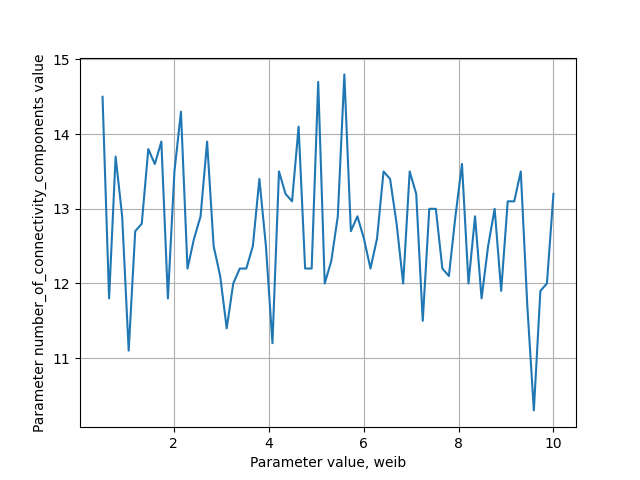
\includegraphics[width=0.7\linewidth]{weib_alpha_knn.png}
    \caption{Зависимость числа компонент связности от $\alpha$ (распределение Weibull)}
    \label{fig:weib_alpha_knn}
\end{figure}

\begin{figure}[H]
    \centering
    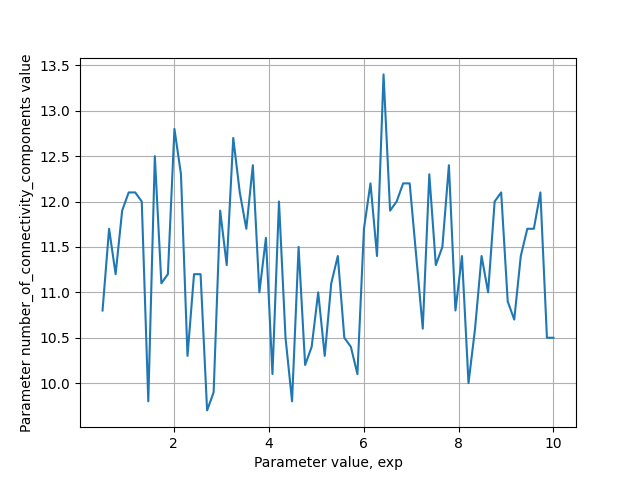
\includegraphics[width=0.7\linewidth]{exp_alpha_knn.png}
    \caption{Зависимость числа компонент связности от $\alpha$ (распределение Exp)}
    \label{fig:exp_alpha_knn}
\end{figure}

Число компонент связности в knn-графах для обоих распределений (рис. \ref{fig:weib_alpha_knn} и \ref{fig:exp_alpha_knn}) слабо зависит от $\alpha$: среднее значение составляет $\approx 12.5$ для Weibull и $\approx 11$ для Exp.

\begin{figure}[H]
    \centering
    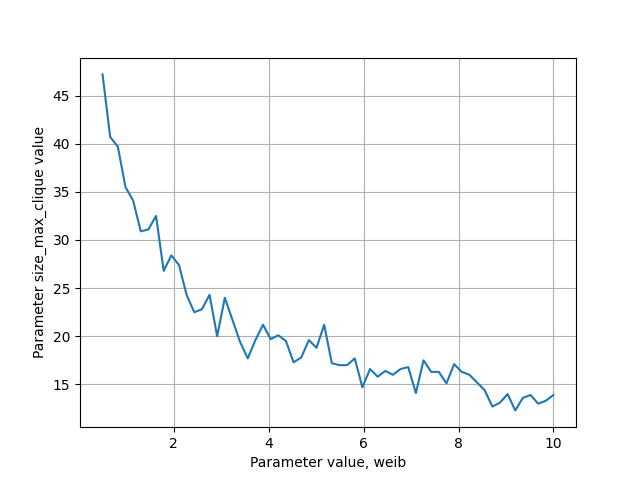
\includegraphics[width=0.7\linewidth]{weib_alpha.png}
    \caption{Зависимость размера максимальной клики от $\alpha$ (Weibull)}
    \label{fig:weib_alpha}
\end{figure}

\begin{figure}[H]
    \centering
    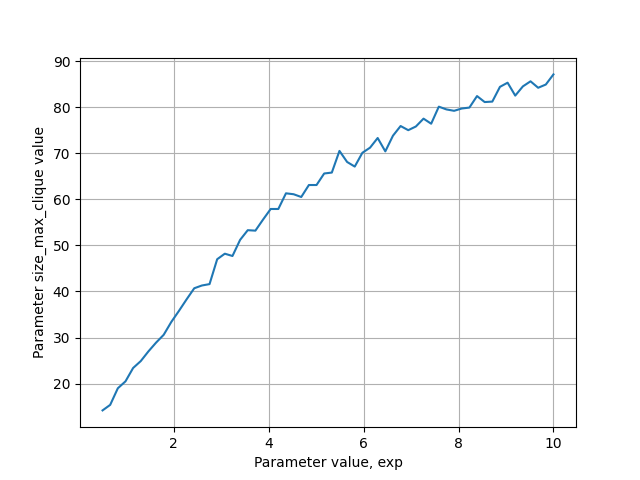
\includegraphics[width=0.7\linewidth]{exp_alpha.png}
    \caption{Зависимость размера максимальной клики от $\alpha$ (Exp)}
    \label{fig:exp_alpha}
\end{figure}

Для размера максимальной клики наблюдается степенная зависимость (рис. \ref{fig:weib_alpha} и \ref{fig:exp_alpha}) с различными показателями степени: $\approx 0.4$ для Weibull и $\approx 0.4$ для Exp.

\begin{figure}[H]
    \centering
    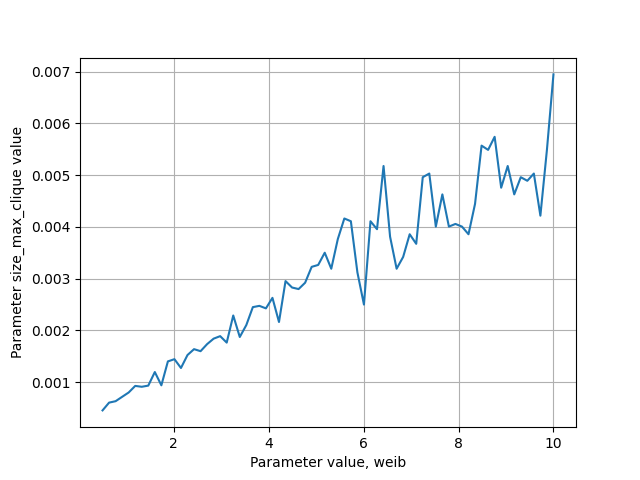
\includegraphics[width=0.7\linewidth]{weib_alpha_fix.png}
    \caption{Выравнивание зависимости максимальной клики от $\alpha$ (Weibull)}
    \label{fig:weib_alpha_fix}
\end{figure}

\begin{figure}[H]
    \centering
    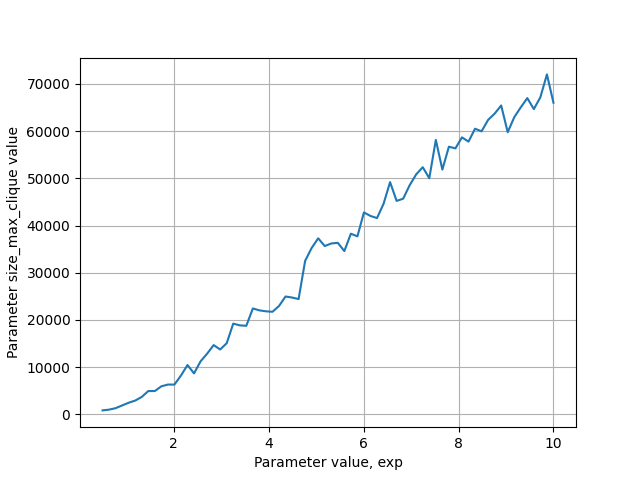
\includegraphics[width=0.7\linewidth]{exp_alpha_fix.png}
    \caption{Выравнивание зависимости максимальной клики от $\alpha$ (Exp)}
    \label{fig:exp_alpha_fix}
\end{figure}

После преобразования степенной зависимостью (рис. \ref{fig:weib_alpha_fix} и \ref{fig:exp_alpha_fix}) получены линейные зависимости, подтверждающие степенной характер.

\section{Пункт 2}

Параметры эксперимента:
\begin{itemize}
    \item $k$: от 2 до 20 (шаг 1)
    \item $d$: от 0.05 до 10 (60 значений)
    \item $n$: от 50 до 100 (шаг 2)
    \item Усреднение по 10 реализациям
\end{itemize}

Основные зависимости:
\begin{enumerate}
    \item От $k$: степенная с отрицательным показателем
    \item От $d$: степенная с показателем $<0$
    \item От $n$: линейная положительная (меньшая дисперсия для кликового числа)
\end{enumerate}

\section{Пункт 3}

Результаты тестирования на выборке $n=300$ (1000 итераций):
\begin{itemize}
    \item \textbf{knn}: power = 0.992, error = 1.0
    \item \textbf{dist}: power = 0.578, error = 1.0
\end{itemize}
Число компонент связности схоже для обоих распределений, кликовое число имеет значительные различия.

\begin{figure}[H]
    \centering
    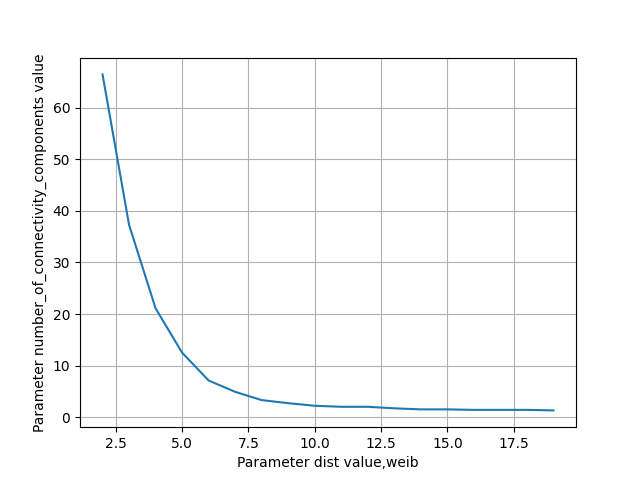
\includegraphics[width=0.45\linewidth]{weib_k.png}
    \hfill
    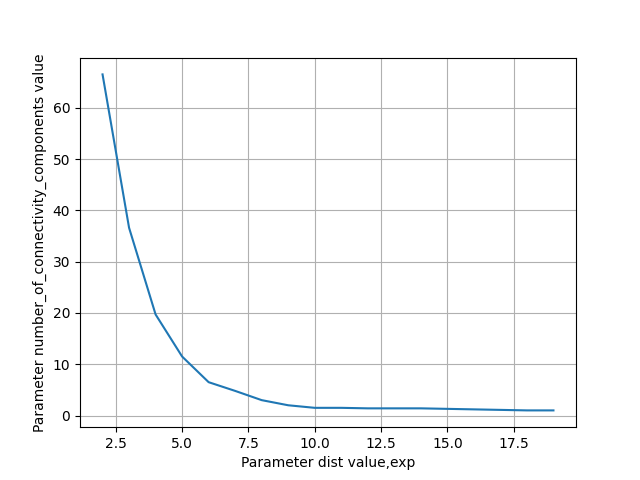
\includegraphics[width=0.45\linewidth]{exp_k.png}
    \caption{Зависимость числа компонент связности от $k$ (Weibull слева, Exp справа)}
    \label{fig:weib_exp_k}
\end{figure}

\begin{figure}[H]
    \centering
    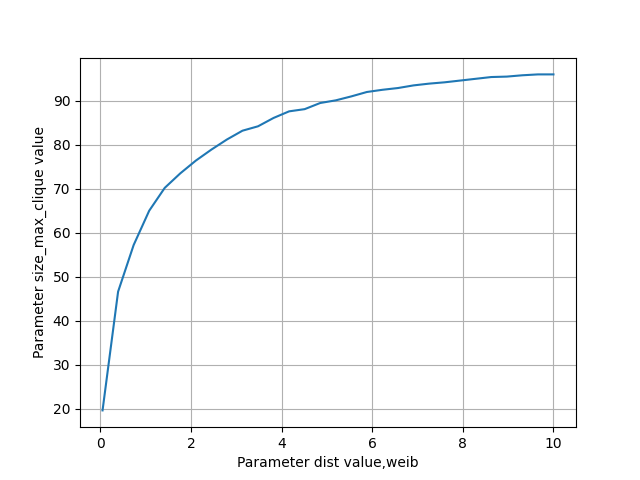
\includegraphics[width=0.45\linewidth]{weib_d.png}
    \hfill
    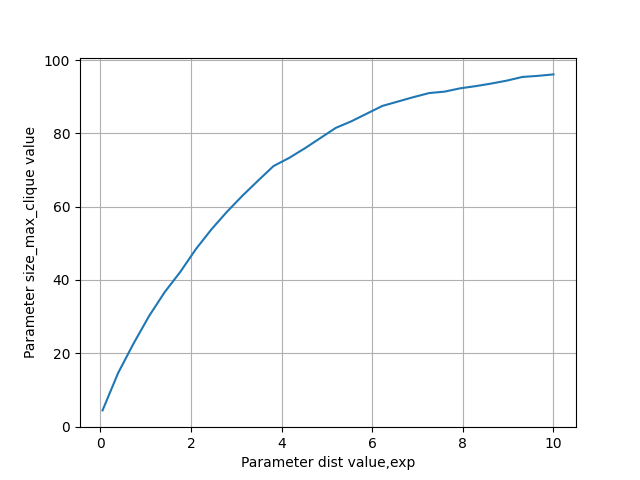
\includegraphics[width=0.45\linewidth]{exp_d.png}
    \caption{Зависимость кликового числа от $d$ (Weibull слева, Exp справа)}
    \label{fig:weib_exp_d}
\end{figure}

\begin{figure}[H]
    \centering
    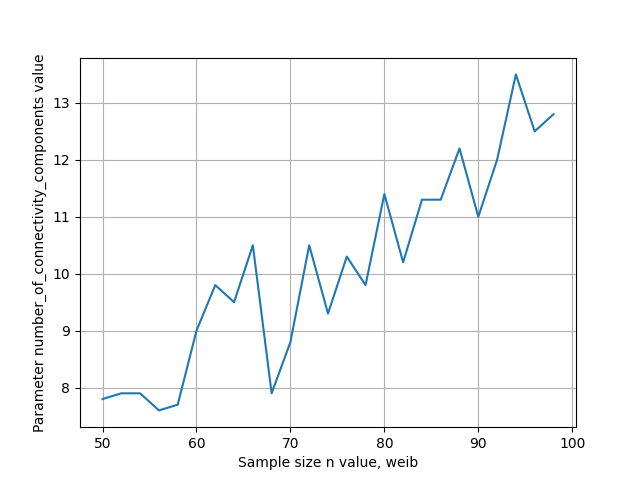
\includegraphics[width=0.45\linewidth]{weib_n_knn.png}
    \hfill
    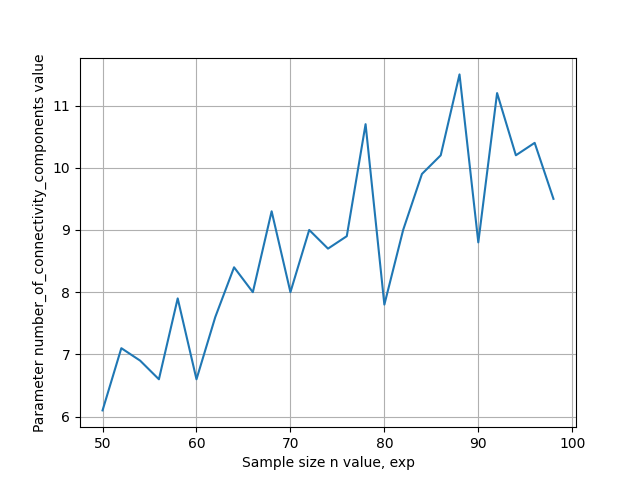
\includegraphics[width=0.45\linewidth]{exp_n_knn.png}
    \caption{Зависимость числа компонент связности от $n$ (Weibull слева, Exp справа)}
    \label{fig:weib_exp_n_knn}
\end{figure}

\begin{figure}[H]
    \centering
    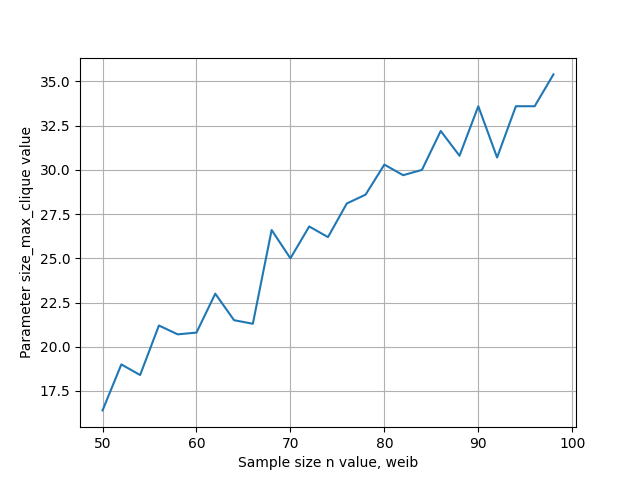
\includegraphics[width=0.45\linewidth]{weib_n.png}
    \hfill
    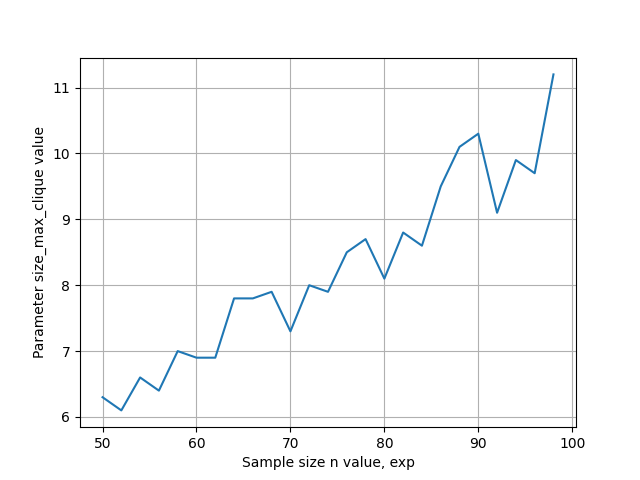
\includegraphics[width=0.45\linewidth]{exp_n.png}
    \caption{Зависимость кликового числа от $n$ (Weibull слева, Exp справа)}
    \label{fig:weib_exp_n}
\end{figure}

\section{Анализ распределений по параметрам}

\subsection{Распределение Student}
\begin{figure}[H]
    \centering
    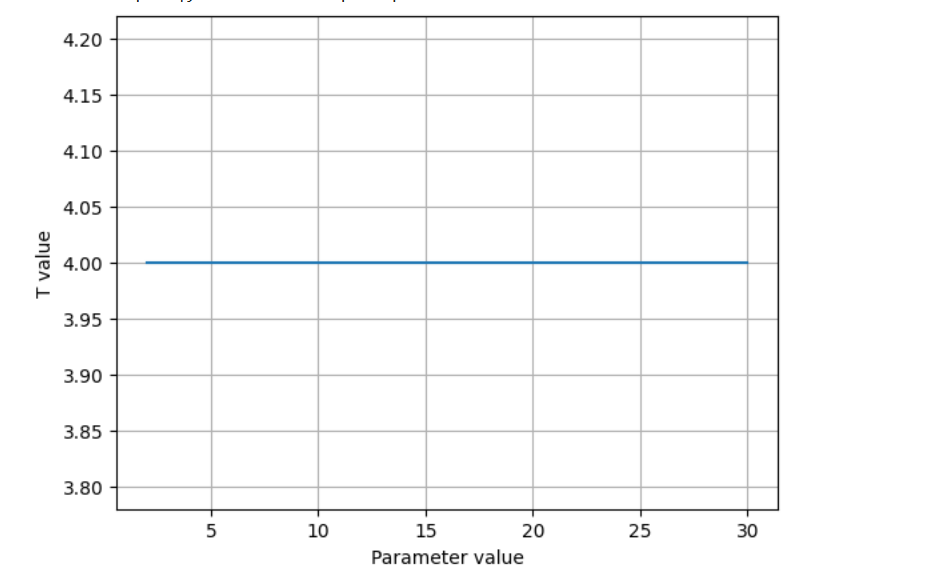
\includegraphics[width=0.7\linewidth]{11.png}
    \caption{Анализ максимальной степени графа (Student)}
    \label{fig:student_param}
\end{figure}
Максимальная степень графа не зависит от параметров распределения.

\subsection{Распределение Laplace}
\begin{figure}[H]
    \centering
    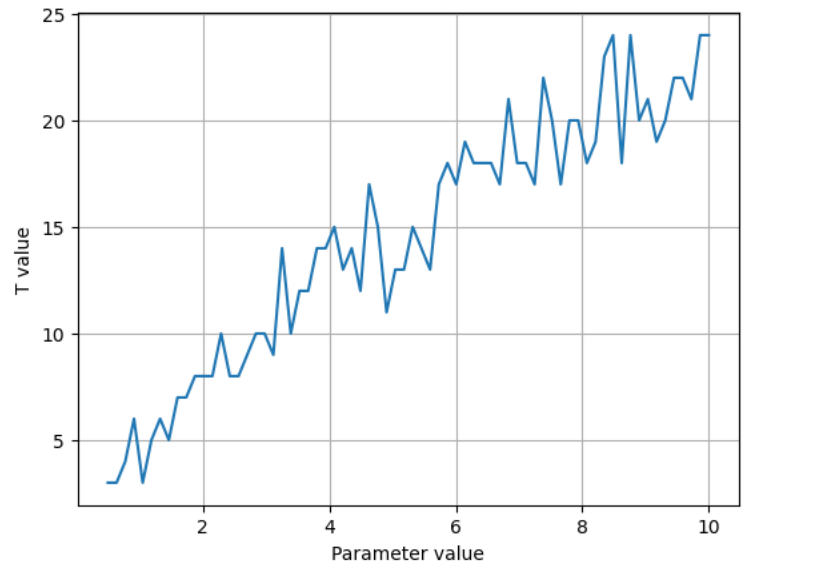
\includegraphics[width=0.7\linewidth]{12.png}
    \caption{Анализ размера максимального независимого множества (Laplace)}
    \label{fig:laplace_param}
\end{figure}
Размер максимального независимого множества прямо пропорционален параметру распределения.

\section{Анализ по $k$ и $d$}

\subsection{Распределение Student ($k$)}
\begin{figure}[H]
    \centering
    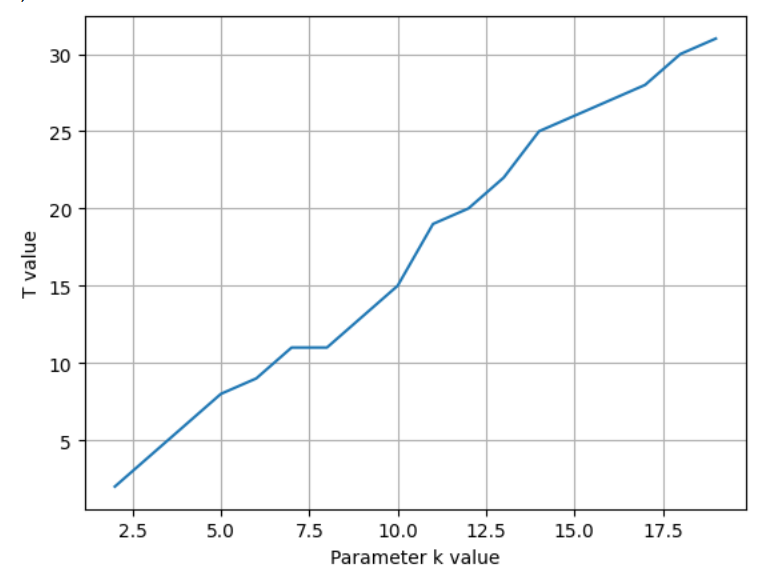
\includegraphics[width=0.7\linewidth]{15.png}
    \caption{Зависимость максимальной степени от $k$ (Student)}
    \label{fig:student_k}
\end{figure}
Линейная зависимость максимальной степени графа от $k$.

\subsection{Распределение Laplace ($d$)}
\begin{figure}[H]
    \centering
    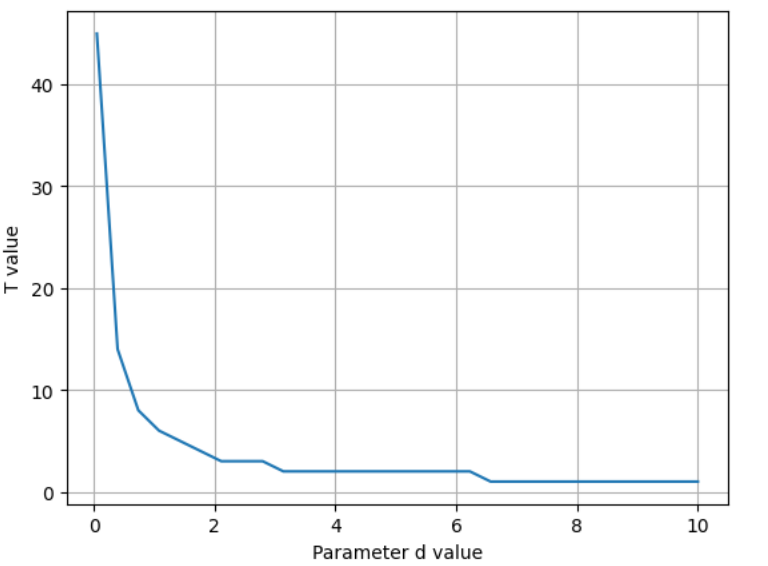
\includegraphics[width=0.7\linewidth]{17.png}
    \caption{Зависимость размера независимого множества от $d$ (Laplace)}
    \label{fig:laplace_d}
\end{figure}
Обратная зависимость размера максимального независимого множества от $d$.

\section{Анализ по выборке $n$}

\subsection{Распределение Student}
\begin{figure}[H]
    \centering
    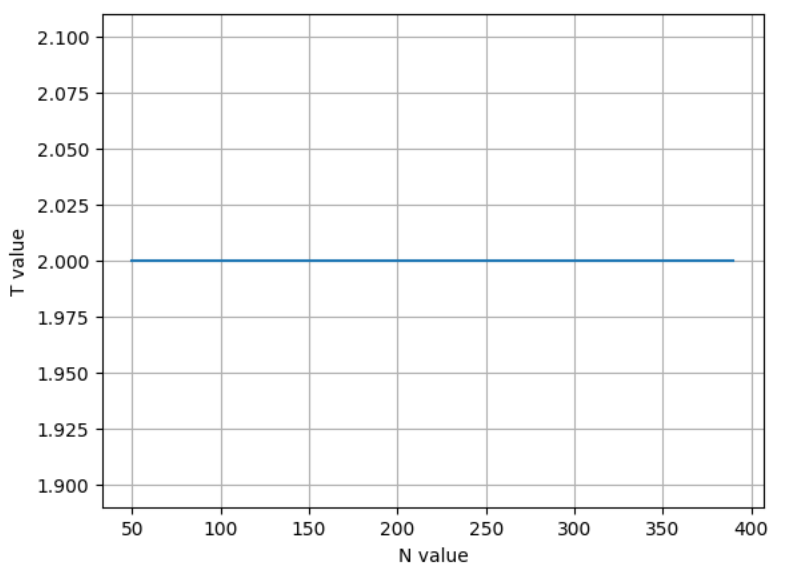
\includegraphics[width=0.7\linewidth]{6.png}
    \caption{Зависимость максимальной степени от $n$ (Student)}
    \label{fig:student_n}
\end{figure}
Отсутствие зависимости от объема выборки.

\subsection{Распределение Laplace}
\begin{figure}[H]
    \centering
    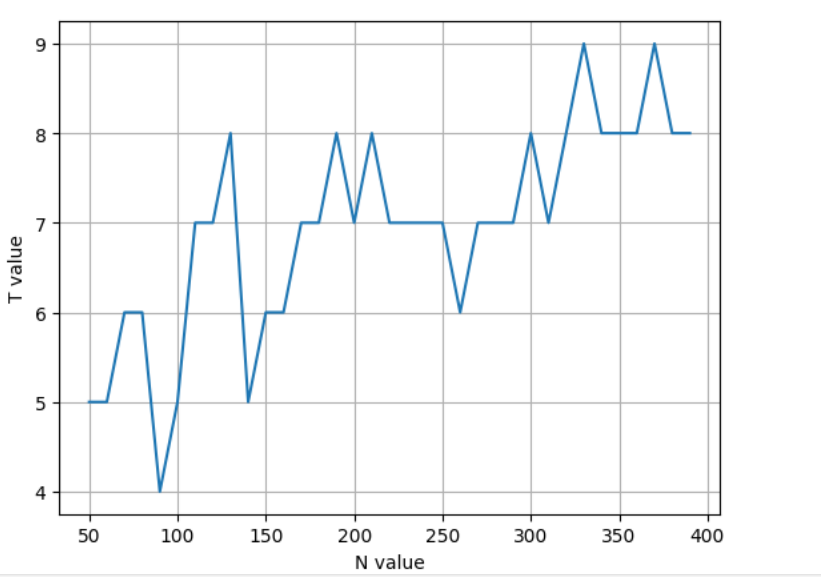
\includegraphics[width=0.7\linewidth]{8.png}
    \caption{Зависимость размера независимого множества от $n$ (Laplace)}
    \label{fig:laplace_n}
\end{figure}
Прямая пропорциональность объему выборки.

\section{Тестирование для Laplace и Student}

Результаты ($n=300$, 1000 итераций):
\begin{itemize}
    \item Мощность критерия: 0.13
    \item Ошибка: 1.0
\end{itemize}
Вероятность ошибочного принятия $H_1$ не превышает 13\%.

\section{Важность характеристик}

\subsection{Student vs Laplace}
\begin{itemize}
    \item \texttt{max\_degree}: 0.6129
    \item \texttt{size\_max\_independent\_set}: 0.3871
\end{itemize}

\subsection{Exp vs Weibull}
\begin{itemize}
    \item \texttt{number\_of\_connectivity\_components}: 0.4483
    \item \texttt{size\_max\_clique}: 0.5517
\end{itemize}

\begin{figure}[H]
    \centering
    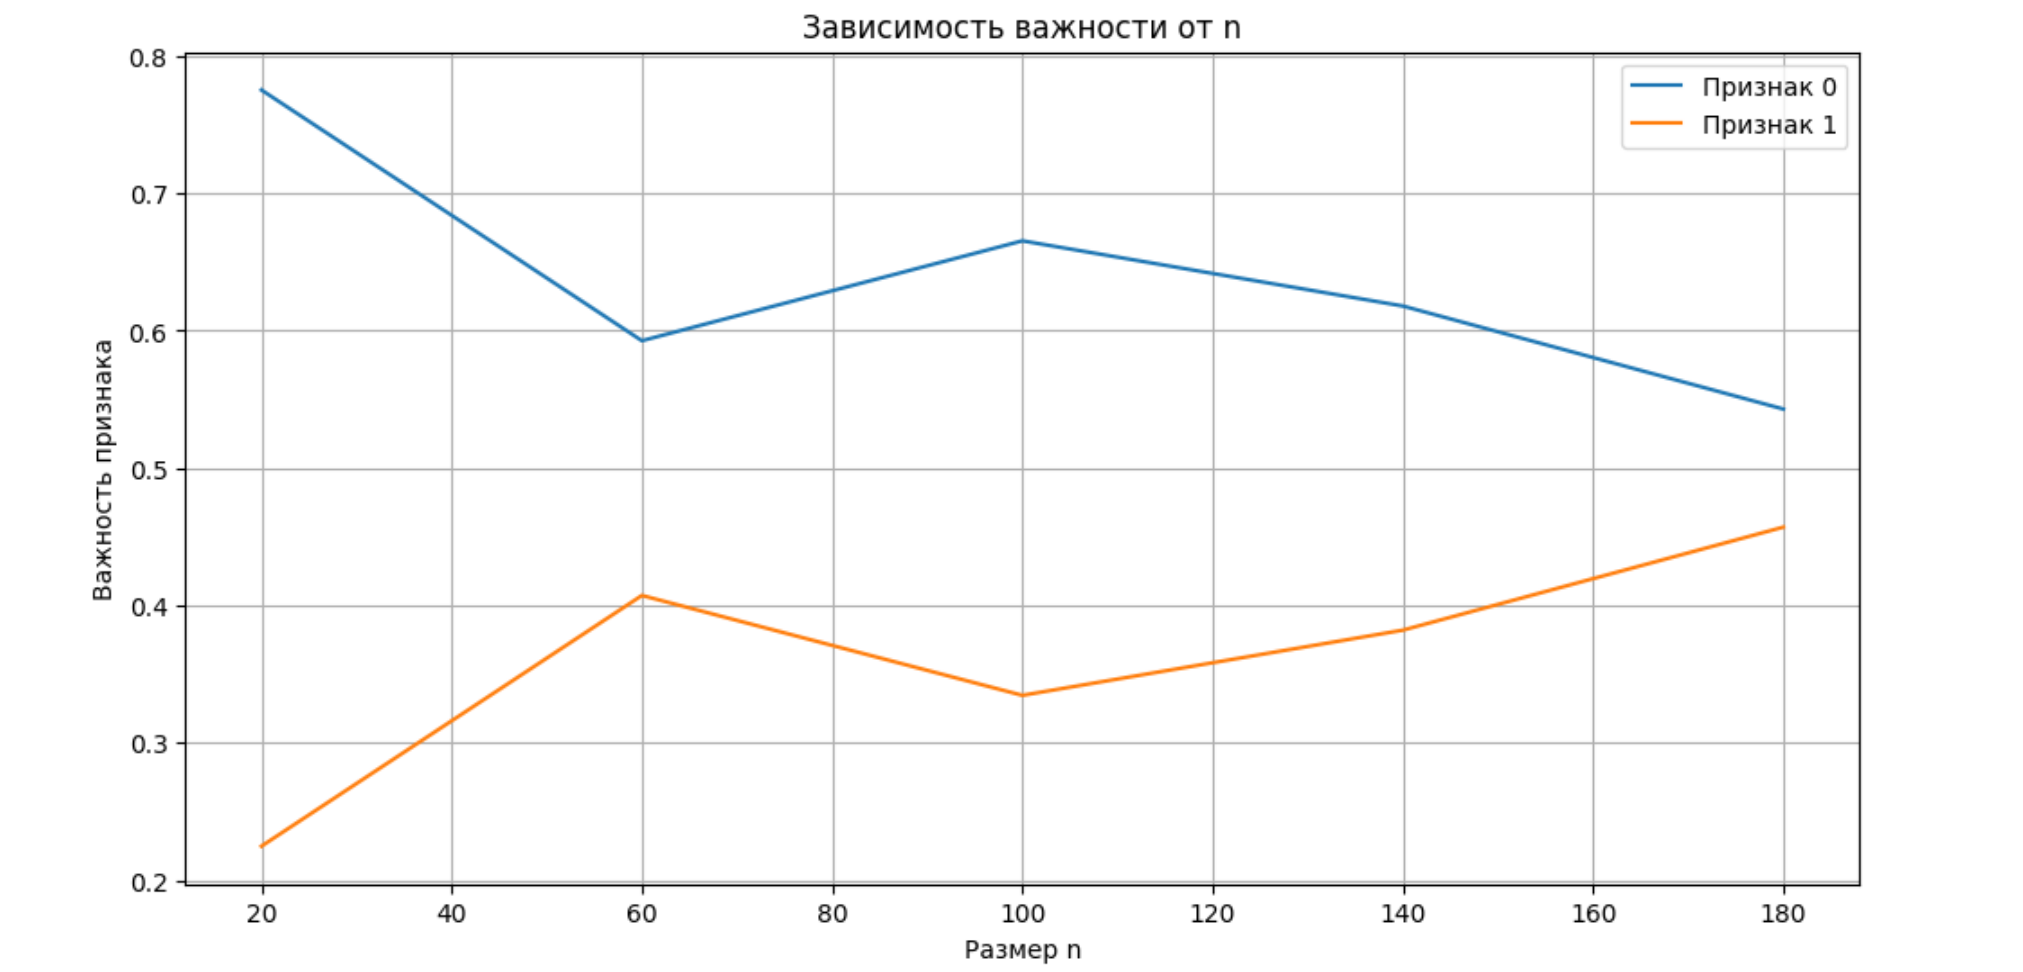
\includegraphics[width=0.7\linewidth]{importance1.png}
    \caption{Важность признаков (Student/Laplace)}
    \label{fig:importance1}
\end{figure}

\begin{figure}[H]
    \centering
    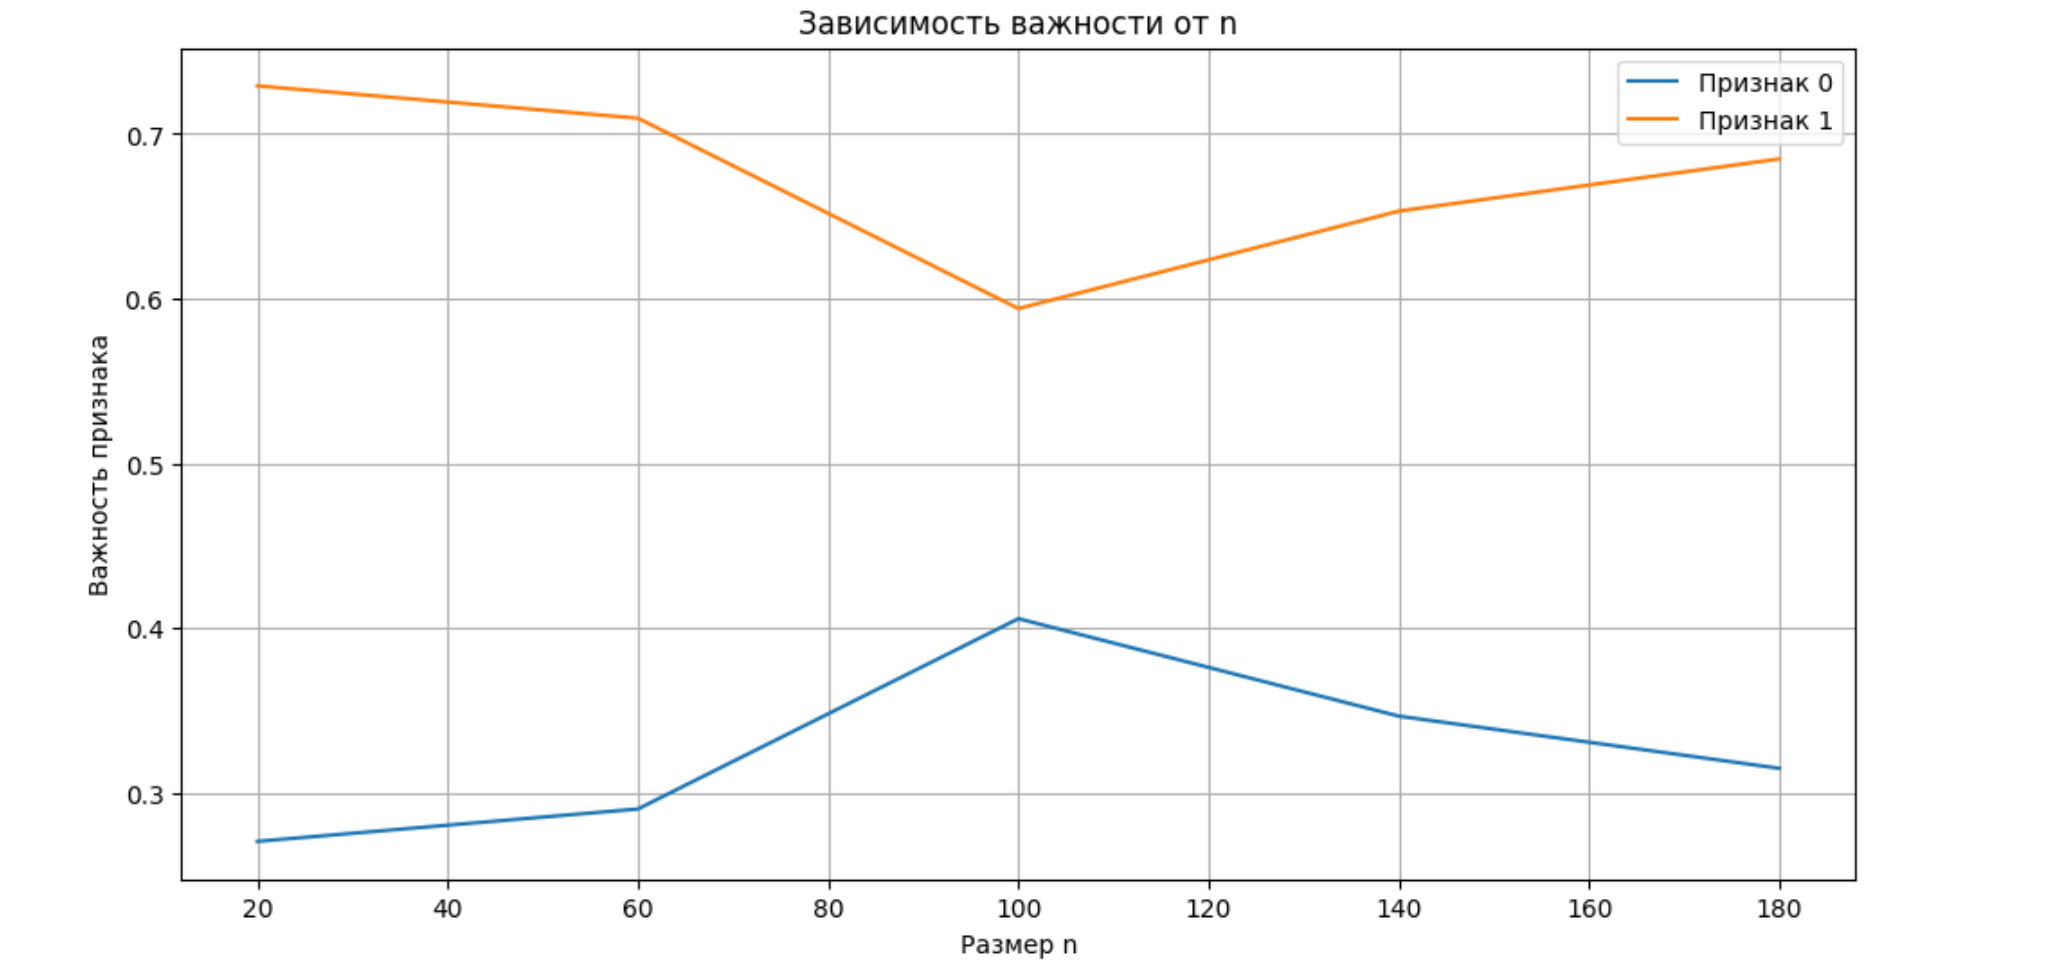
\includegraphics[width=0.7\linewidth]{importance2.png}
    \caption{Важность признаков (Exp/Weibull)}
    \label{fig:importance2}
\end{figure}

Выводы:
\begin{itemize}
    \item Для Student/Laplace ключевой признак — максимальная степень графа
    \item Для Exp/Weibull ключевой признак — число компонент связности
\end{itemize}

\section{Анализ метрик}

\subsection{Student vs Laplace}
\begin{itemize}
    \item При малых $n$: лучший метод — kNN
    \item При больших $n$: точность = 1 для всех методов
    \item Ошибка I рода: 0.5
    \item Мощность: 0.5
    \item Точность: 1.0
\end{itemize}

\subsection{Exp vs Weibull}
\begin{itemize}
    \item При малых $n$: лучшие методы — Логистическая регрессия и kNN
    \item При больших $n$: лучшие методы — Дерево решений и Логистическая регрессия
    \item Ошибка I рода: 0.02
    \item Мощность: 0.23
    \item Точность: 0.71
\end{itemize}

\begin{figure}[H]
    \centering
    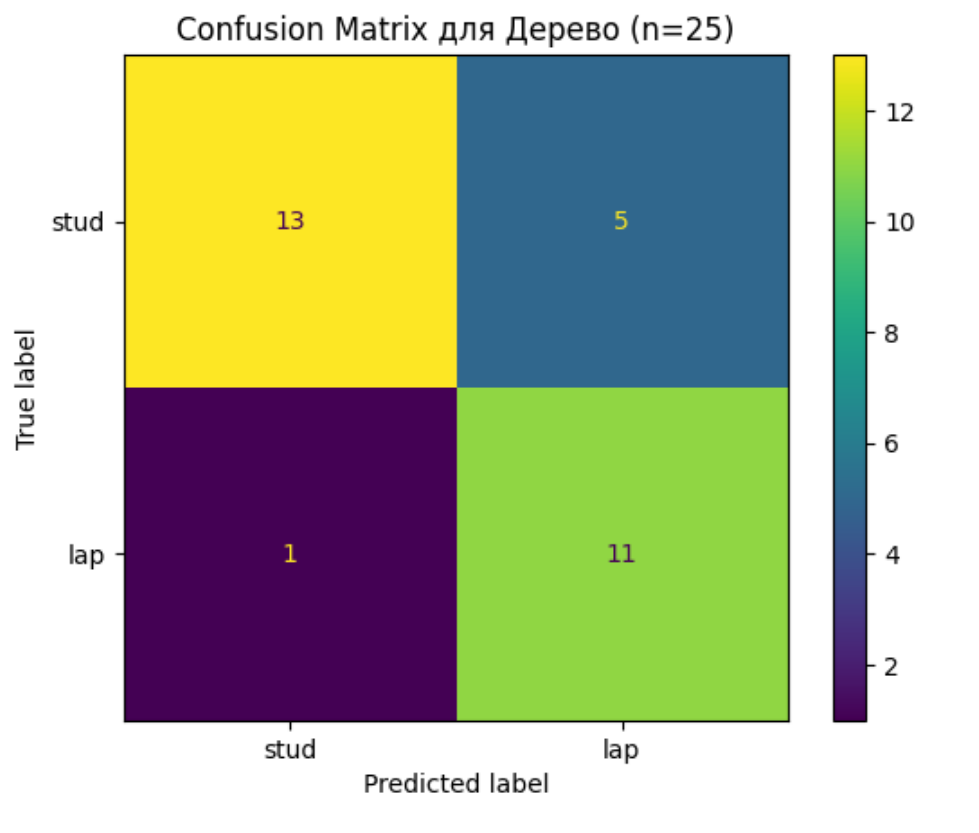
\includegraphics[width=0.45\linewidth]{Confusion matrix lap and stud 1.png}
    \hfill
    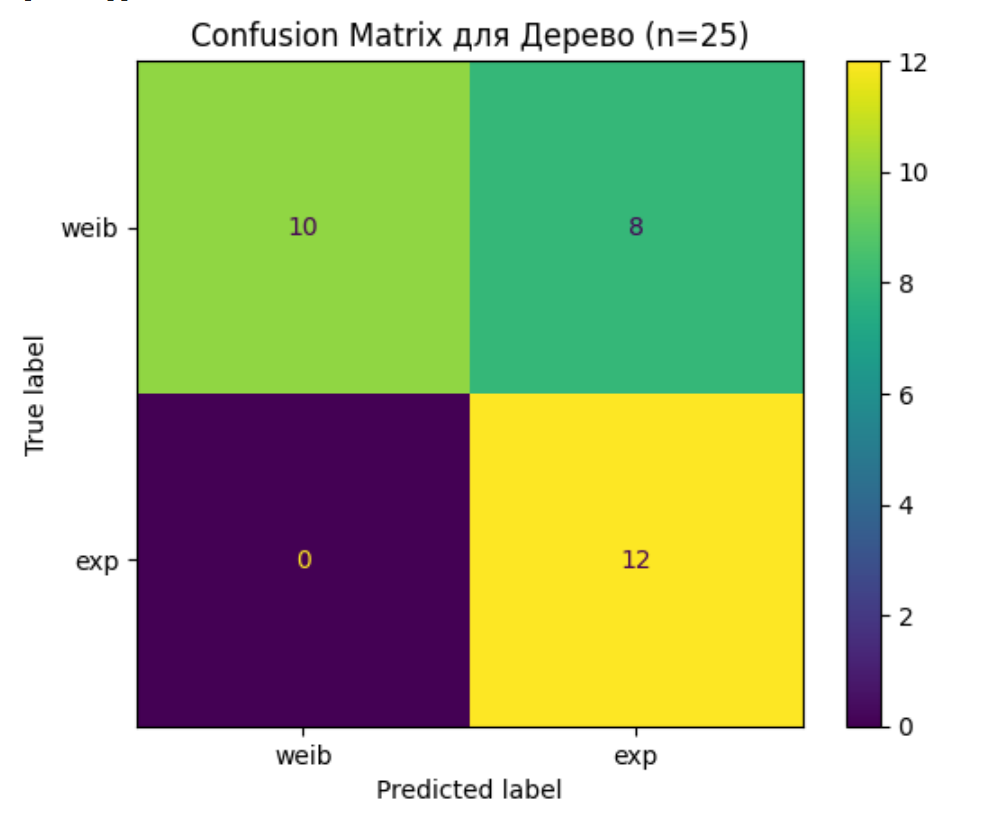
\includegraphics[width=0.45\linewidth]{Confusion matrix weih and exp 1.png}
    \caption{Матрицы ошибок для $n=25$ (слева: Student/Laplace, справа: Exp/Weibull)}
    \label{fig:cm25}
\end{figure}

\begin{figure}[H]
    \centering
    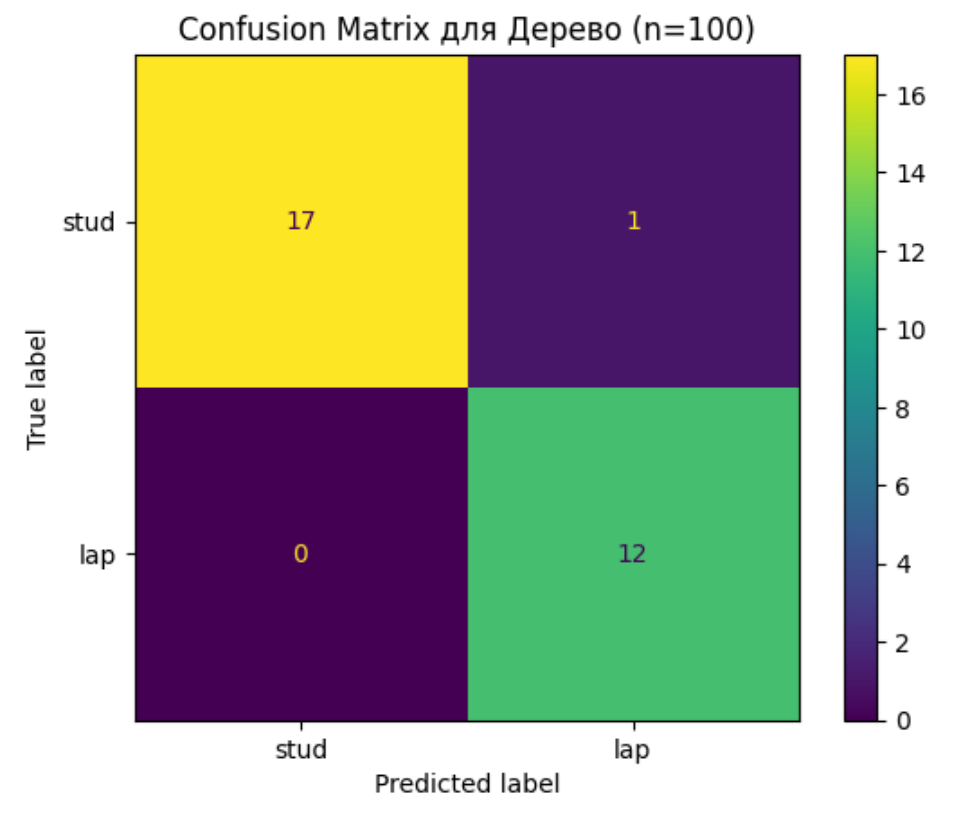
\includegraphics[width=0.45\linewidth]{Confusion matrix lap and stud 2.png}
    \hfill
    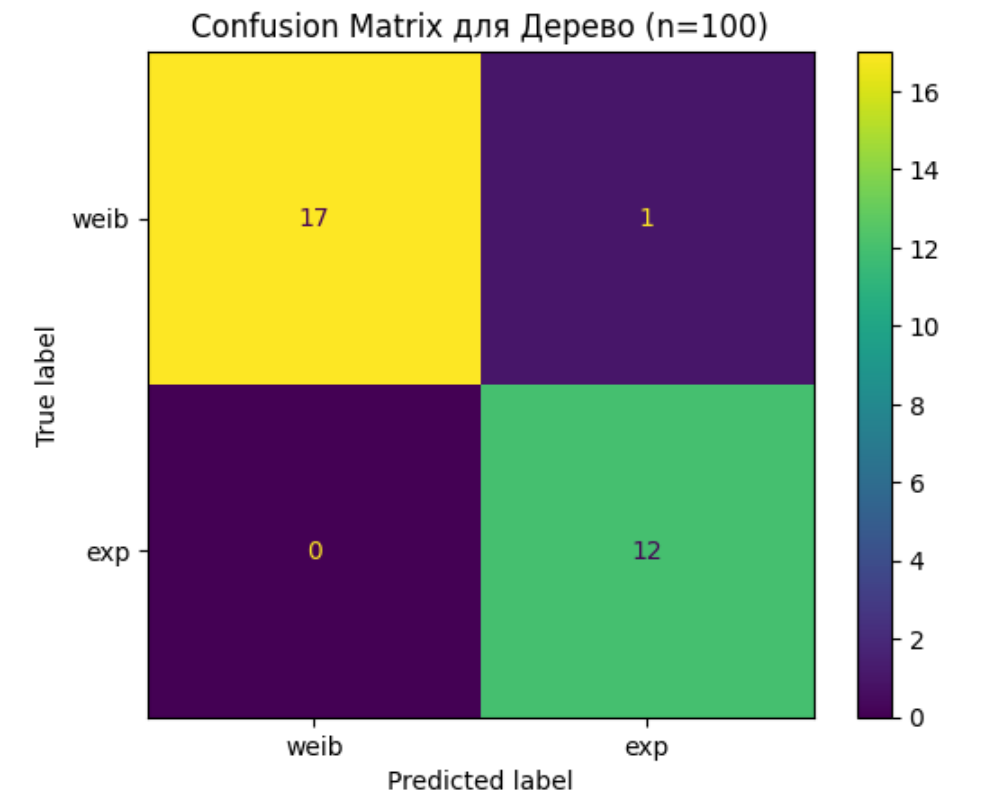
\includegraphics[width=0.45\linewidth]{Confusion matrix weih and exp 2.png}
    \caption{Матрицы ошибок для $n=100$}
    \label{fig:cm100}
\end{figure}

\begin{figure}[H]
    \centering
    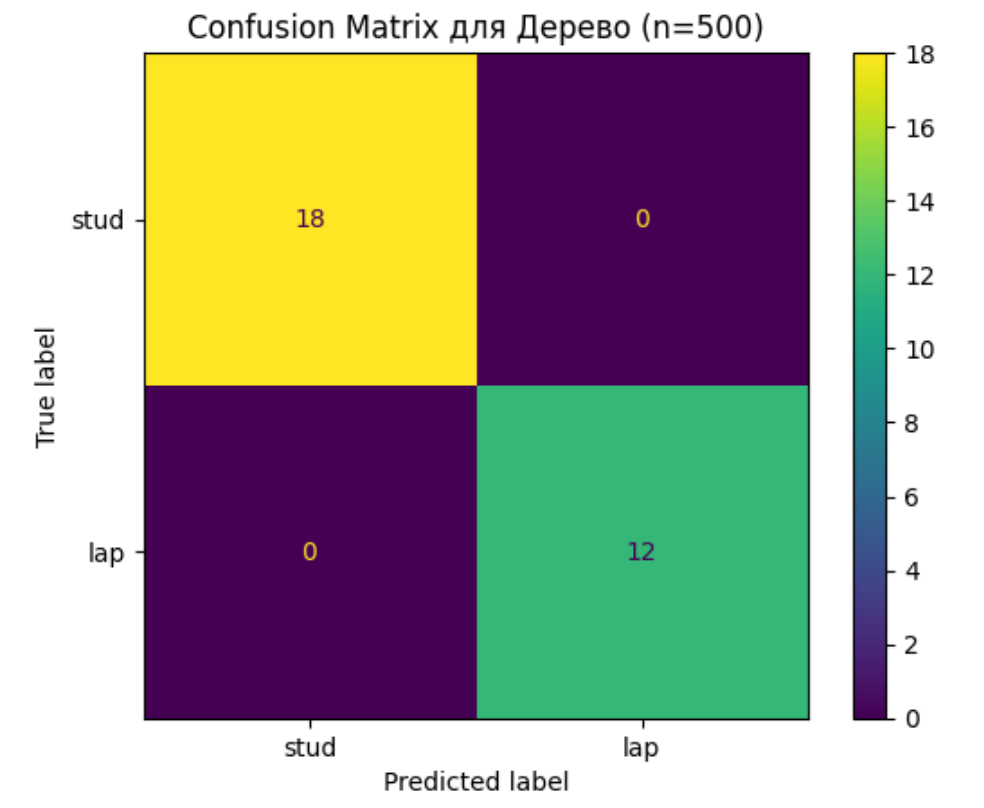
\includegraphics[width=0.45\linewidth]{Confusion matrix lap and stud 3.png}
    \hfill
    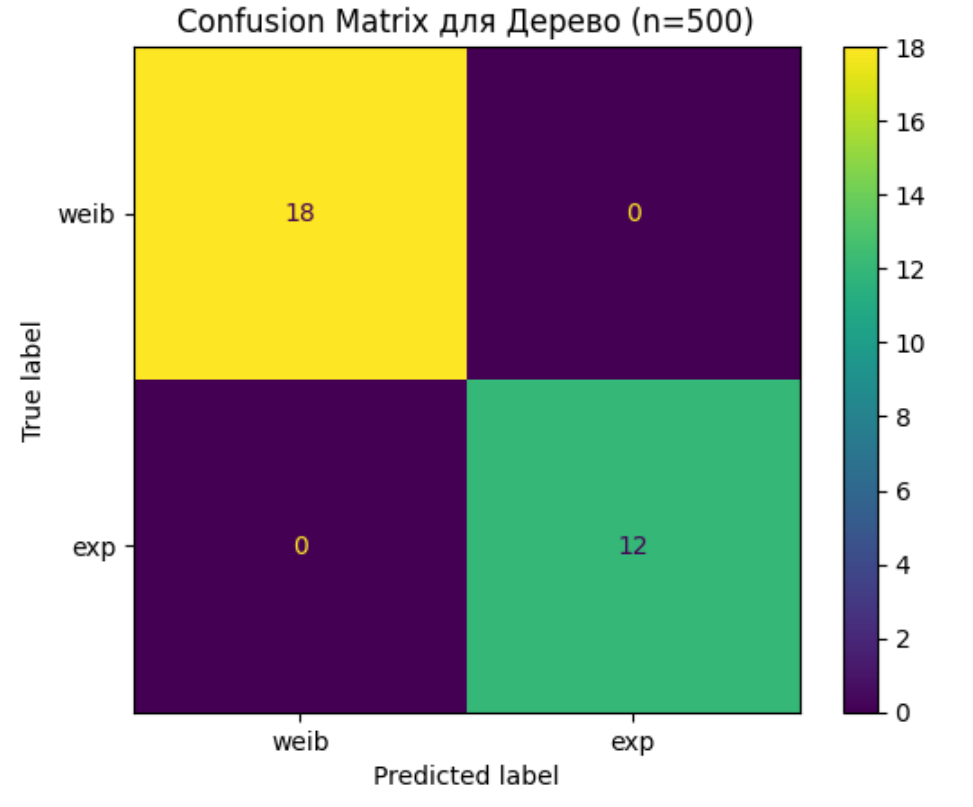
\includegraphics[width=0.45\linewidth]{Confusion matrix weih and exp 3.png}
    \caption{Матрицы ошибок для $n=500$}
    \label{fig:cm500}
\end{figure}

\section*{Реализация}
\begin{itemize}
    \item \textbf{Часть 1}
    \begin{itemize}
        \item Создание gd: Лев
        \item Создание gk: Илья
        \item Пункт 1: Лев, Илья
        \item Пункт 2: Лев, Илья
        \item Пункт 3: Илья
    \end{itemize}
    
    \item \textbf{Часть 2}
    \begin{itemize}
        \item Пункты 1-2: Лев
        \item Пункт 3: Илья
    \end{itemize}
\end{itemize}

\end{document}